\documentclass[10pt,twoside]{article}
\usepackage[utf8]{inputenc}
\usepackage{amsmath}
\usepackage{amsfonts}
\usepackage{amssymb}
\usepackage[spanish,es-noshorthands]{babel}
\usepackage[T1]{fontenc}
\usepackage{lmodern}
\usepackage{graphicx,hyperref}
\usepackage{tikz,pgf}
\usepackage{multicol}
\usepackage{subfig}
\usepackage[papersize={6.5in,8.5in},width=5.5in,height=7in]{geometry}
\usepackage{fancyhdr}
\pagestyle{fancy}
\fancyhead[LE]{
\includegraphics[height=12pt]{Images/logo-colegio.png} Aritmética $6^{\circ}$}
\fancyhead[RE]{}
\fancyhead[RO]{\textit{Germ\'an Avenda\~no Ram\'irez, Lic. U.D., M.Sc. U.N.}}
\fancyhead[LO]{}

\author{Germ\'an Avenda\~no Ram\'irez, Lic. U.D., M.Sc. U.N.}
\title{\begin{minipage}{.2\textwidth}

\includegraphics[height=1.75cm]{Images/logo-colegio.png}\end{minipage}
\begin{minipage}{.55\textwidth}
\begin{center}
Taller 11, Múltiplos y divisores \\
Aritmética $6^{\circ}$
\end{center}
\end{minipage}\hfill
\begin{minipage}{.2\textwidth}

\includegraphics[height=1.75cm]{Images/logo-sed.png} 
\end{minipage}}
\date{}
\begin{document}
\maketitle
Nombre: \hrulefill Curso: \underline{\hspace*{44pt}} Fecha: \underline{\hspace*{2.5cm}}\\

\begin{minipage}{.3\textwidth}
El siguiente esquema, muesta la manera en que se relacionan los conceptos de esta unidad.
\section*{Explora tus conocimientos}
Javier y su hermano, tienen una pequeña casa en la colina de una montaña. Allí tiene 4 vacas y un caballo. Diariamente los jóvenes ordeñan sus vacas y de cada una sacan dos litros de leche.
\end{minipage}
\begin{minipage}{.7\textwidth}
\ifx\du\undefined
  \newlength{\du}
\fi
\setlength{\du}{15\unitlength}
\begin{tikzpicture}[scale=.65]
\pgftransformxscale{1.000000}
\pgftransformyscale{-1.000000}
\definecolor{dialinecolor}{rgb}{0.000000, 0.000000, 0.000000}
\pgfsetstrokecolor{dialinecolor}
\definecolor{dialinecolor}{rgb}{1.000000, 1.000000, 1.000000}
\pgfsetfillcolor{dialinecolor}
% setfont left to latex
\definecolor{dialinecolor}{rgb}{0.000000, 0.000000, 0.000000}
\pgfsetstrokecolor{dialinecolor}
\node[anchor=west] at (13.250000\du,5.750000\du){};
% setfont left to latex
\definecolor{dialinecolor}{rgb}{0.000000, 0.000000, 0.000000}
\pgfsetstrokecolor{dialinecolor}
\node[anchor=west] at (20.300000\du,5.250000\du){Presentan};
\pgfsetlinewidth{0.100000\du}
\pgfsetdash{}{0pt}
\pgfsetdash{}{0pt}
\pgfsetbuttcap
{
\definecolor{dialinecolor}{rgb}{0.000000, 0.000000, 0.000000}
\pgfsetfillcolor{dialinecolor}
% was here!!!
\definecolor{dialinecolor}{rgb}{0.000000, 0.000000, 0.000000}
\pgfsetstrokecolor{dialinecolor}
\draw (21.564569\du,3.749960\du)--(21.600000\du,4.712500\du);
}
\pgfsetlinewidth{0.100000\du}
\pgfsetdash{}{0pt}
\pgfsetdash{}{0pt}
\pgfsetbuttcap
{
\definecolor{dialinecolor}{rgb}{0.000000, 0.000000, 0.000000}
\pgfsetfillcolor{dialinecolor}
% was here!!!
\pgfsetarrowsend{to}
\definecolor{dialinecolor}{rgb}{0.000000, 0.000000, 0.000000}
\pgfsetstrokecolor{dialinecolor}
\draw (21.550000\du,5.512500\du)--(21.616010\du,6.799686\du);
}
\pgfsetlinewidth{0.100000\du}
\pgfsetdash{}{0pt}
\pgfsetdash{}{0pt}
\pgfsetbuttcap
\pgfsetmiterjoin
\pgfsetlinewidth{0.100000\du}
\pgfsetbuttcap
\pgfsetmiterjoin
\pgfsetdash{}{0pt}
\definecolor{dialinecolor}{rgb}{1.000000, 1.000000, 1.000000}
\pgfsetfillcolor{dialinecolor}
\pgfpathmoveto{\pgfpoint{17.268750\du}{6.687500\du}}
\pgfpathlineto{\pgfpoint{25.881250\du}{6.687500\du}}
\pgfpathcurveto{\pgfpoint{27.070389\du}{6.687500\du}}{\pgfpoint{28.034375\du}{7.193978\du}}{\pgfpoint{28.034375\du}{7.818750\du}}
\pgfpathcurveto{\pgfpoint{28.034375\du}{8.443522\du}}{\pgfpoint{27.070389\du}{8.950000\du}}{\pgfpoint{25.881250\du}{8.950000\du}}
\pgfpathlineto{\pgfpoint{17.268750\du}{8.950000\du}}
\pgfpathcurveto{\pgfpoint{16.079611\du}{8.950000\du}}{\pgfpoint{15.115625\du}{8.443522\du}}{\pgfpoint{15.115625\du}{7.818750\du}}
\pgfpathcurveto{\pgfpoint{15.115625\du}{7.193978\du}}{\pgfpoint{16.079611\du}{6.687500\du}}{\pgfpoint{17.268750\du}{6.687500\du}}
\pgfusepath{fill}
\definecolor{dialinecolor}{rgb}{0.000000, 0.000000, 0.000000}
\pgfsetstrokecolor{dialinecolor}
\pgfpathmoveto{\pgfpoint{17.268750\du}{6.687500\du}}
\pgfpathlineto{\pgfpoint{25.881250\du}{6.687500\du}}
\pgfpathcurveto{\pgfpoint{27.070389\du}{6.687500\du}}{\pgfpoint{28.034375\du}{7.193978\du}}{\pgfpoint{28.034375\du}{7.818750\du}}
\pgfpathcurveto{\pgfpoint{28.034375\du}{8.443522\du}}{\pgfpoint{27.070389\du}{8.950000\du}}{\pgfpoint{25.881250\du}{8.950000\du}}
\pgfpathlineto{\pgfpoint{17.268750\du}{8.950000\du}}
\pgfpathcurveto{\pgfpoint{16.079611\du}{8.950000\du}}{\pgfpoint{15.115625\du}{8.443522\du}}{\pgfpoint{15.115625\du}{7.818750\du}}
\pgfpathcurveto{\pgfpoint{15.115625\du}{7.193978\du}}{\pgfpoint{16.079611\du}{6.687500\du}}{\pgfpoint{17.268750\du}{6.687500\du}}
\pgfusepath{stroke}
% setfont left to latex
\definecolor{dialinecolor}{rgb}{0.000000, 0.000000, 0.000000}
\pgfsetstrokecolor{dialinecolor}
\node at (21.575000\du,8.018750\du){Relaciones multiplicativas};
% setfont left to latex
\definecolor{dialinecolor}{rgb}{0.000000, 0.000000, 0.000000}
\pgfsetstrokecolor{dialinecolor}
\node[anchor=west] at (21.575000\du,7.818750\du){};
\pgfsetlinewidth{0.100000\du}
\pgfsetdash{}{0pt}
\pgfsetdash{}{0pt}
\pgfsetbuttcap
\pgfsetmiterjoin
\pgfsetlinewidth{0.100000\du}
\pgfsetbuttcap
\pgfsetmiterjoin
\pgfsetdash{}{0pt}
\definecolor{dialinecolor}{rgb}{1.000000, 1.000000, 1.000000}
\pgfsetfillcolor{dialinecolor}
\pgfpathmoveto{\pgfpoint{16.998750\du}{1.650000\du}}
\pgfpathlineto{\pgfpoint{26.051250\du}{1.650000\du}}
\pgfpathcurveto{\pgfpoint{27.301140\du}{1.650000\du}}{\pgfpoint{28.314375\du}{2.108908\du}}{\pgfpoint{28.314375\du}{2.675000\du}}
\pgfpathcurveto{\pgfpoint{28.314375\du}{3.241092\du}}{\pgfpoint{27.301140\du}{3.700000\du}}{\pgfpoint{26.051250\du}{3.700000\du}}
\pgfpathlineto{\pgfpoint{16.998750\du}{3.700000\du}}
\pgfpathcurveto{\pgfpoint{15.748860\du}{3.700000\du}}{\pgfpoint{14.735625\du}{3.241092\du}}{\pgfpoint{14.735625\du}{2.675000\du}}
\pgfpathcurveto{\pgfpoint{14.735625\du}{2.108908\du}}{\pgfpoint{15.748860\du}{1.650000\du}}{\pgfpoint{16.998750\du}{1.650000\du}}
\pgfusepath{fill}
\definecolor{dialinecolor}{rgb}{0.000000, 0.000000, 0.000000}
\pgfsetstrokecolor{dialinecolor}
\pgfpathmoveto{\pgfpoint{16.998750\du}{1.650000\du}}
\pgfpathlineto{\pgfpoint{26.051250\du}{1.650000\du}}
\pgfpathcurveto{\pgfpoint{27.301140\du}{1.650000\du}}{\pgfpoint{28.314375\du}{2.108908\du}}{\pgfpoint{28.314375\du}{2.675000\du}}
\pgfpathcurveto{\pgfpoint{28.314375\du}{3.241092\du}}{\pgfpoint{27.301140\du}{3.700000\du}}{\pgfpoint{26.051250\du}{3.700000\du}}
\pgfpathlineto{\pgfpoint{16.998750\du}{3.700000\du}}
\pgfpathcurveto{\pgfpoint{15.748860\du}{3.700000\du}}{\pgfpoint{14.735625\du}{3.241092\du}}{\pgfpoint{14.735625\du}{2.675000\du}}
\pgfpathcurveto{\pgfpoint{14.735625\du}{2.108908\du}}{\pgfpoint{15.748860\du}{1.650000\du}}{\pgfpoint{16.998750\du}{1.650000\du}}
\pgfusepath{stroke}
% setfont left to latex
\definecolor{dialinecolor}{rgb}{0.000000, 0.000000, 0.000000}
\pgfsetstrokecolor{dialinecolor}
\node at (21.525000\du,2.914712\du){Los números naturales};
\pgfsetlinewidth{0.100000\du}
\pgfsetdash{}{0pt}
\pgfsetdash{}{0pt}
\pgfsetbuttcap
{
\definecolor{dialinecolor}{rgb}{0.000000, 0.000000, 0.000000}
\pgfsetfillcolor{dialinecolor}
% was here!!!
\definecolor{dialinecolor}{rgb}{0.000000, 0.000000, 0.000000}
\pgfsetstrokecolor{dialinecolor}
\draw (21.607263\du,8.999045\du)--(21.650000\du,10.562500\du);
}
% setfont left to latex
\definecolor{dialinecolor}{rgb}{0.000000, 0.000000, 0.000000}
\pgfsetstrokecolor{dialinecolor}
\node[anchor=west] at (20.800000\du,11.312500\du){como};
\pgfsetlinewidth{0.100000\du}
\pgfsetdash{}{0pt}
\pgfsetdash{}{0pt}
\pgfsetbuttcap
{
\definecolor{dialinecolor}{rgb}{0.000000, 0.000000, 0.000000}
\pgfsetfillcolor{dialinecolor}
% was here!!!
\pgfsetarrowsend{to}
\definecolor{dialinecolor}{rgb}{0.000000, 0.000000, 0.000000}
\pgfsetstrokecolor{dialinecolor}
\draw (21.650000\du,11.612500\du)--(21.625000\du,13.050000\du);
}
\pgfsetlinewidth{0.100000\du}
\pgfsetdash{}{0pt}
\pgfsetdash{}{0pt}
\pgfsetbuttcap
{
\definecolor{dialinecolor}{rgb}{0.000000, 0.000000, 0.000000}
\pgfsetfillcolor{dialinecolor}
% was here!!!
\definecolor{dialinecolor}{rgb}{0.000000, 0.000000, 0.000000}
\pgfsetstrokecolor{dialinecolor}
\draw (16.500000\du,13.050000\du)--(26.750000\du,13.050000\du);
}
\pgfsetlinewidth{0.100000\du}
\pgfsetdash{}{0pt}
\pgfsetdash{}{0pt}
\pgfsetbuttcap
{
\definecolor{dialinecolor}{rgb}{0.000000, 0.000000, 0.000000}
\pgfsetfillcolor{dialinecolor}
% was here!!!
\definecolor{dialinecolor}{rgb}{0.000000, 0.000000, 0.000000}
\pgfsetstrokecolor{dialinecolor}
\draw (16.600000\du,13.087500\du)--(16.549658\du,14.150970\du);
}
\pgfsetlinewidth{0.100000\du}
\pgfsetdash{}{0pt}
\pgfsetdash{}{0pt}
\pgfsetbuttcap
\pgfsetmiterjoin
\pgfsetlinewidth{0.100000\du}
\pgfsetbuttcap
\pgfsetmiterjoin
\pgfsetdash{}{0pt}
\definecolor{dialinecolor}{rgb}{1.000000, 1.000000, 1.000000}
\pgfsetfillcolor{dialinecolor}
\pgfpathmoveto{\pgfpoint{13.503750\du}{14.200000\du}}
\pgfpathlineto{\pgfpoint{19.496250\du}{14.200000\du}}
\pgfpathcurveto{\pgfpoint{20.323642\du}{14.200000\du}}{\pgfpoint{20.994375\du}{14.647715\du}}{\pgfpoint{20.994375\du}{15.200000\du}}
\pgfpathcurveto{\pgfpoint{20.994375\du}{15.752285\du}}{\pgfpoint{20.323642\du}{16.200000\du}}{\pgfpoint{19.496250\du}{16.200000\du}}
\pgfpathlineto{\pgfpoint{13.503750\du}{16.200000\du}}
\pgfpathcurveto{\pgfpoint{12.676358\du}{16.200000\du}}{\pgfpoint{12.005625\du}{15.752285\du}}{\pgfpoint{12.005625\du}{15.200000\du}}
\pgfpathcurveto{\pgfpoint{12.005625\du}{14.647715\du}}{\pgfpoint{12.676358\du}{14.200000\du}}{\pgfpoint{13.503750\du}{14.200000\du}}
\pgfusepath{fill}
\definecolor{dialinecolor}{rgb}{0.000000, 0.000000, 0.000000}
\pgfsetstrokecolor{dialinecolor}
\pgfpathmoveto{\pgfpoint{13.503750\du}{14.200000\du}}
\pgfpathlineto{\pgfpoint{19.496250\du}{14.200000\du}}
\pgfpathcurveto{\pgfpoint{20.323642\du}{14.200000\du}}{\pgfpoint{20.994375\du}{14.647715\du}}{\pgfpoint{20.994375\du}{15.200000\du}}
\pgfpathcurveto{\pgfpoint{20.994375\du}{15.752285\du}}{\pgfpoint{20.323642\du}{16.200000\du}}{\pgfpoint{19.496250\du}{16.200000\du}}
\pgfpathlineto{\pgfpoint{13.503750\du}{16.200000\du}}
\pgfpathcurveto{\pgfpoint{12.676358\du}{16.200000\du}}{\pgfpoint{12.005625\du}{15.752285\du}}{\pgfpoint{12.005625\du}{15.200000\du}}
\pgfpathcurveto{\pgfpoint{12.005625\du}{14.647715\du}}{\pgfpoint{12.676358\du}{14.200000\du}}{\pgfpoint{13.503750\du}{14.200000\du}}
\pgfusepath{stroke}
% setfont left to latex
\definecolor{dialinecolor}{rgb}{0.000000, 0.000000, 0.000000}
\pgfsetstrokecolor{dialinecolor}
\node at (16.500000\du,15.400000\du){Ser múltiplo de ...};
\pgfsetlinewidth{0.100000\du}
\pgfsetdash{}{0pt}
\pgfsetdash{}{0pt}
\pgfsetbuttcap
\pgfsetmiterjoin
\pgfsetlinewidth{0.100000\du}
\pgfsetbuttcap
\pgfsetmiterjoin
\pgfsetdash{}{0pt}
\definecolor{dialinecolor}{rgb}{1.000000, 1.000000, 1.000000}
\pgfsetfillcolor{dialinecolor}
\pgfpathmoveto{\pgfpoint{23.943750\du}{14.300000\du}}
\pgfpathlineto{\pgfpoint{29.456250\du}{14.300000\du}}
\pgfpathcurveto{\pgfpoint{30.217368\du}{14.300000\du}}{\pgfpoint{30.834375\du}{14.736522\du}}{\pgfpoint{30.834375\du}{15.275000\du}}
\pgfpathcurveto{\pgfpoint{30.834375\du}{15.813478\du}}{\pgfpoint{30.217368\du}{16.250000\du}}{\pgfpoint{29.456250\du}{16.250000\du}}
\pgfpathlineto{\pgfpoint{23.943750\du}{16.250000\du}}
\pgfpathcurveto{\pgfpoint{23.182632\du}{16.250000\du}}{\pgfpoint{22.565625\du}{15.813478\du}}{\pgfpoint{22.565625\du}{15.275000\du}}
\pgfpathcurveto{\pgfpoint{22.565625\du}{14.736522\du}}{\pgfpoint{23.182632\du}{14.300000\du}}{\pgfpoint{23.943750\du}{14.300000\du}}
\pgfusepath{fill}
\definecolor{dialinecolor}{rgb}{0.000000, 0.000000, 0.000000}
\pgfsetstrokecolor{dialinecolor}
\pgfpathmoveto{\pgfpoint{23.943750\du}{14.300000\du}}
\pgfpathlineto{\pgfpoint{29.456250\du}{14.300000\du}}
\pgfpathcurveto{\pgfpoint{30.217368\du}{14.300000\du}}{\pgfpoint{30.834375\du}{14.736522\du}}{\pgfpoint{30.834375\du}{15.275000\du}}
\pgfpathcurveto{\pgfpoint{30.834375\du}{15.813478\du}}{\pgfpoint{30.217368\du}{16.250000\du}}{\pgfpoint{29.456250\du}{16.250000\du}}
\pgfpathlineto{\pgfpoint{23.943750\du}{16.250000\du}}
\pgfpathcurveto{\pgfpoint{23.182632\du}{16.250000\du}}{\pgfpoint{22.565625\du}{15.813478\du}}{\pgfpoint{22.565625\du}{15.275000\du}}
\pgfpathcurveto{\pgfpoint{22.565625\du}{14.736522\du}}{\pgfpoint{23.182632\du}{14.300000\du}}{\pgfpoint{23.943750\du}{14.300000\du}}
\pgfusepath{stroke}
% setfont left to latex
\definecolor{dialinecolor}{rgb}{0.000000, 0.000000, 0.000000}
\pgfsetstrokecolor{dialinecolor}
\node at (26.700000\du,15.475000\du){Ser divisor de ...};
\pgfsetlinewidth{0.100000\du}
\pgfsetdash{}{0pt}
\pgfsetdash{}{0pt}
\pgfsetbuttcap
{
\definecolor{dialinecolor}{rgb}{0.000000, 0.000000, 0.000000}
\pgfsetfillcolor{dialinecolor}
% was here!!!
\definecolor{dialinecolor}{rgb}{0.000000, 0.000000, 0.000000}
\pgfsetstrokecolor{dialinecolor}
\draw (26.700000\du,12.987500\du)--(26.700000\du,14.250763\du);
}
\pgfsetlinewidth{0.100000\du}
\pgfsetdash{}{0pt}
\pgfsetdash{}{0pt}
\pgfsetbuttcap
{
\definecolor{dialinecolor}{rgb}{0.000000, 0.000000, 0.000000}
\pgfsetfillcolor{dialinecolor}
% was here!!!
\definecolor{dialinecolor}{rgb}{0.000000, 0.000000, 0.000000}
\pgfsetstrokecolor{dialinecolor}
\draw (26.700000\du,16.300089\du)--(26.700000\du,17.937500\du);
}
% setfont left to latex
\definecolor{dialinecolor}{rgb}{0.000000, 0.000000, 0.000000}
\pgfsetstrokecolor{dialinecolor}
\node[anchor=west] at (25.100000\du,18.537500\du){determina};
\pgfsetlinewidth{0.100000\du}
\pgfsetdash{}{0pt}
\pgfsetdash{}{0pt}
\pgfsetbuttcap
{
\definecolor{dialinecolor}{rgb}{0.000000, 0.000000, 0.000000}
\pgfsetfillcolor{dialinecolor}
% was here!!!
\pgfsetarrowsend{to}
\definecolor{dialinecolor}{rgb}{0.000000, 0.000000, 0.000000}
\pgfsetstrokecolor{dialinecolor}
\draw (26.700000\du,18.687500\du)--(26.775000\du,20.412500\du);
}
\pgfsetlinewidth{0.100000\du}
\pgfsetdash{}{0pt}
\pgfsetdash{}{0pt}
\pgfsetbuttcap
{
\definecolor{dialinecolor}{rgb}{0.000000, 0.000000, 0.000000}
\pgfsetfillcolor{dialinecolor}
% was here!!!
\definecolor{dialinecolor}{rgb}{0.000000, 0.000000, 0.000000}
\pgfsetstrokecolor{dialinecolor}
\draw (21.750000\du,20.437500\du)--(31.800000\du,20.387500\du);
}
\pgfsetlinewidth{0.100000\du}
\pgfsetdash{}{0pt}
\pgfsetdash{}{0pt}
\pgfsetbuttcap
{
\definecolor{dialinecolor}{rgb}{0.000000, 0.000000, 0.000000}
\pgfsetfillcolor{dialinecolor}
% was here!!!
\definecolor{dialinecolor}{rgb}{0.000000, 0.000000, 0.000000}
\pgfsetstrokecolor{dialinecolor}
\draw (21.850000\du,20.487500\du)--(21.876843\du,21.437080\du);
}
\pgfsetlinewidth{0.100000\du}
\pgfsetdash{}{0pt}
\pgfsetdash{}{0pt}
\pgfsetbuttcap
\pgfsetmiterjoin
\pgfsetlinewidth{0.100000\du}
\pgfsetbuttcap
\pgfsetmiterjoin
\pgfsetdash{}{0pt}
\definecolor{dialinecolor}{rgb}{1.000000, 1.000000, 1.000000}
\pgfsetfillcolor{dialinecolor}
\pgfpathmoveto{\pgfpoint{19.113750\du}{21.487500\du}}
\pgfpathlineto{\pgfpoint{24.686250\du}{21.487500\du}}
\pgfpathcurveto{\pgfpoint{25.455652\du}{21.487500\du}}{\pgfpoint{26.079375\du}{21.831681\du}}{\pgfpoint{26.079375\du}{22.256250\du}}
\pgfpathcurveto{\pgfpoint{26.079375\du}{22.680819\du}}{\pgfpoint{25.455652\du}{23.025000\du}}{\pgfpoint{24.686250\du}{23.025000\du}}
\pgfpathlineto{\pgfpoint{19.113750\du}{23.025000\du}}
\pgfpathcurveto{\pgfpoint{18.344348\du}{23.025000\du}}{\pgfpoint{17.720625\du}{22.680819\du}}{\pgfpoint{17.720625\du}{22.256250\du}}
\pgfpathcurveto{\pgfpoint{17.720625\du}{21.831681\du}}{\pgfpoint{18.344348\du}{21.487500\du}}{\pgfpoint{19.113750\du}{21.487500\du}}
\pgfusepath{fill}
\definecolor{dialinecolor}{rgb}{0.000000, 0.000000, 0.000000}
\pgfsetstrokecolor{dialinecolor}
\pgfpathmoveto{\pgfpoint{19.113750\du}{21.487500\du}}
\pgfpathlineto{\pgfpoint{24.686250\du}{21.487500\du}}
\pgfpathcurveto{\pgfpoint{25.455652\du}{21.487500\du}}{\pgfpoint{26.079375\du}{21.831681\du}}{\pgfpoint{26.079375\du}{22.256250\du}}
\pgfpathcurveto{\pgfpoint{26.079375\du}{22.680819\du}}{\pgfpoint{25.455652\du}{23.025000\du}}{\pgfpoint{24.686250\du}{23.025000\du}}
\pgfpathlineto{\pgfpoint{19.113750\du}{23.025000\du}}
\pgfpathcurveto{\pgfpoint{18.344348\du}{23.025000\du}}{\pgfpoint{17.720625\du}{22.680819\du}}{\pgfpoint{17.720625\du}{22.256250\du}}
\pgfpathcurveto{\pgfpoint{17.720625\du}{21.831681\du}}{\pgfpoint{18.344348\du}{21.487500\du}}{\pgfpoint{19.113750\du}{21.487500\du}}
\pgfusepath{stroke}
% setfont left to latex
\definecolor{dialinecolor}{rgb}{0.000000, 0.000000, 0.000000}
\pgfsetstrokecolor{dialinecolor}
\node at (21.900000\du,22.456250\du){Números primos};
\pgfsetlinewidth{0.100000\du}
\pgfsetdash{}{0pt}
\pgfsetdash{}{0pt}
\pgfsetbuttcap
\pgfsetmiterjoin
\pgfsetlinewidth{0.100000\du}
\pgfsetbuttcap
\pgfsetmiterjoin
\pgfsetdash{}{0pt}
\definecolor{dialinecolor}{rgb}{1.000000, 1.000000, 1.000000}
\pgfsetfillcolor{dialinecolor}
\pgfpathmoveto{\pgfpoint{28.320000\du}{21.487500\du}}
\pgfpathlineto{\pgfpoint{35.580000\du}{21.487500\du}}
\pgfpathcurveto{\pgfpoint{36.582397\du}{21.487500\du}}{\pgfpoint{37.395000\du}{21.868058\du}}{\pgfpoint{37.395000\du}{22.337500\du}}
\pgfpathcurveto{\pgfpoint{37.395000\du}{22.806942\du}}{\pgfpoint{36.582397\du}{23.187500\du}}{\pgfpoint{35.580000\du}{23.187500\du}}
\pgfpathlineto{\pgfpoint{28.320000\du}{23.187500\du}}
\pgfpathcurveto{\pgfpoint{27.317603\du}{23.187500\du}}{\pgfpoint{26.505000\du}{22.806942\du}}{\pgfpoint{26.505000\du}{22.337500\du}}
\pgfpathcurveto{\pgfpoint{26.505000\du}{21.868058\du}}{\pgfpoint{27.317603\du}{21.487500\du}}{\pgfpoint{28.320000\du}{21.487500\du}}
\pgfusepath{fill}
\definecolor{dialinecolor}{rgb}{0.000000, 0.000000, 0.000000}
\pgfsetstrokecolor{dialinecolor}
\pgfpathmoveto{\pgfpoint{28.320000\du}{21.487500\du}}
\pgfpathlineto{\pgfpoint{35.580000\du}{21.487500\du}}
\pgfpathcurveto{\pgfpoint{36.582397\du}{21.487500\du}}{\pgfpoint{37.395000\du}{21.868058\du}}{\pgfpoint{37.395000\du}{22.337500\du}}
\pgfpathcurveto{\pgfpoint{37.395000\du}{22.806942\du}}{\pgfpoint{36.582397\du}{23.187500\du}}{\pgfpoint{35.580000\du}{23.187500\du}}
\pgfpathlineto{\pgfpoint{28.320000\du}{23.187500\du}}
\pgfpathcurveto{\pgfpoint{27.317603\du}{23.187500\du}}{\pgfpoint{26.505000\du}{22.806942\du}}{\pgfpoint{26.505000\du}{22.337500\du}}
\pgfpathcurveto{\pgfpoint{26.505000\du}{21.868058\du}}{\pgfpoint{27.317603\du}{21.487500\du}}{\pgfpoint{28.320000\du}{21.487500\du}}
\pgfusepath{stroke}
% setfont left to latex
\definecolor{dialinecolor}{rgb}{0.000000, 0.000000, 0.000000}
\pgfsetstrokecolor{dialinecolor}
\node at (31.950000\du,22.537500\du){Números compuestos};
\pgfsetlinewidth{0.100000\du}
\pgfsetdash{}{0pt}
\pgfsetdash{}{0pt}
\pgfsetbuttcap
{
\definecolor{dialinecolor}{rgb}{0.000000, 0.000000, 0.000000}
\pgfsetfillcolor{dialinecolor}
% was here!!!
\definecolor{dialinecolor}{rgb}{0.000000, 0.000000, 0.000000}
\pgfsetstrokecolor{dialinecolor}
\draw (31.850000\du,20.487500\du)--(31.901343\du,21.437341\du);
}
\end{tikzpicture}
\end{minipage}
\begin{itemize}
\item ¿Cuántos litros de leche recogen al ordeñar la primera vaca?
\item ¿Cuántos litros de leche en total recogen cuando terminan de ordeñar la segunda vaca?
\item ¿Cuántos litros de leche en total tienen cuándo terminan de ordenar la tercera vaca?
\item ¿Cuántos litros de leche en total reúnen cuando terminan de ordeñar la cuarta vaca?
\item Completa en tu cuaderno la siguiente tabla.
\end{itemize}
\begin{center}
\begin{tabular}{|p{3cm}|c|c|c|c|}
\hline 
\textbf{Vaca ordeñada} & \textbf{Primera} & \textbf{Segunda} & \textbf{Tercera} & \textbf{Cuarta} \\ 
\hline 
Cantidad de leche en litros en total &  &  &  &  \\ 
\hline 
\end{tabular} 
\end{center}
\begin{itemize}
\item ¿Qué procedimiento seguiste para completar la tabla?
\end{itemize}
\section*{Lo que s\'{e}}
\subsection*{¿Sabes que es un reptil?}
\subsubsection*{¿Alguna vez has visto alguno?}
Sabes que en Colombia hay criaderos de reptiles que se
encuentran ubicados en zonas templadas o calientes. En esos
criaderos se encuentran diferentes especies de culebras, lagartos, tortugas, cocodrilos, y otros más.
\begin{itemize}
\item Juan trabaja en uno de esos criaderos de reptiles. Él debe recoger, cada semana, los huevos que colocan las hembras, para llevarlos a un sitio seguro y caliente.
\item En esta ocasión recogió los huevos de 16 culebras ratoneras. Ellas colocan entre 3 y 45 huevos, en los meses de junio y agosto.

\begin{minipage}{.35\textwidth}
\item Juan pasó por cada uno de los 16 terrarios recogiendo los huevos. En el primer terrario, no había huevos, en el segundo, recogió 3 huevos, en el tercero, 6 huevos, en el cuarto, 9 huevos, en el quinto, Juan encontró 12 huevos, y así sucesivamente.
\item Escribe la secuencia numérica que se forma con la cantidad de huevos que recogió Juan en cada terrario.
\end{minipage}\hfill
\begin{minipage}{.65\textwidth}
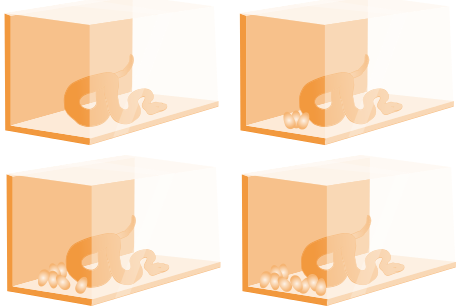
\includegraphics[scale=.5]{Images/culebras.png} 
\end{minipage}
\end{itemize}
\section*{Aprendo algo nuevo}
Responde en tu cuaderno
\begin{itemize}
\item ¿Qué procedimiento seguiste para completar la
secuencia anterior?
\item ¿Qué relación hay entre los números que escribiste?
\item ¿Cuántos huevos hay en el sexto terrario?
\item ¿Cuántos huevos hay en el noveno terrario?
\item ¿Cómo hallaste ese resultado?
\item ¿En qué terrario hay 42 huevos?
\item ¿Cómo hallaste la respuesta?
\end{itemize}
Completa en tu cuaderno el siguiente diagrama

\begin{tikzpicture}
[level distance=10mm,
every node/.style={fill=red!60,circle,inner sep=1pt},
level 1/.style={sibling distance=16mm,nodes={fill=red!45}},
level 2/.style={sibling distance=8mm,nodes={fill=red!30}},
level 3/.style={sibling distance=4mm,nodes={fill=red!25}}]
\node {\textbf{3}}
child {node {$\times$}
child {node{0}
child {node{0}}}
child {node{1}
child {node{3}}}
child {node{2}
child {node{6}}}
child {node{3}
child {node{?}}}
child {node{4}
child {node{?}}}
child {node{5}
child {node{?}}}
child {node{6}
child {node{?}}}
child {node{7}
child {node{?}}}
child {node{8}
child {node{?}}}
child {node{9}
child {node{?}}}
child {node{10}
child {node{?}}}
child {node{11}
child {node{?}}}
child {node{12}
child {node{?}}}
child {node{13}
child {node{?}}}
child {node{14}
child {node{?}}}
child {node{15}
child {node{?}}}
child {node{16}
child {node{?}}}
};
\end{tikzpicture}
\begin{itemize}
\item ¿Los resultados que obtuviste en el árbol, son
iguales a la secuencia que escribiste en la actividad
inicial?
\end{itemize}
Los números que escribiste en la actividad inicial y los
obtenidos en el árbol son los múltiplos de 3.
\begin{itemize}
\item ¿Cómo se hallan los múltiplos de 3? Añade otras ramas a tu árbol, y encuentra otros múltiplos de 3.
\item ¿Este conjunto de múltiplos tiene último elemento?
¿Por qué?
\item ¿Los múltiplos de 3, se dividen exactamente por 3?
Compruébalo realizando algunas divisiones.
\end{itemize}
Juan organiza cada grupo de huevos de las culebras ratoneras, en bandejas, para guardarlos en la incubadora del criadero de reptiles. Para guardar el grupo de 24 huevos encuentra varias bandejas.
\begin{center}
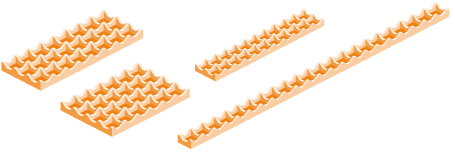
\includegraphics[scale=.75]{Images/huevos.png} 
\end{center}
\begin{itemize}
\item ¿Cuáles son las posibles distribuciones que puede hacer
Juan con los 24 huevos?
\item En tu cuaderno completa el siguiente diagrama.

\begin{minipage}{.4\textwidth}
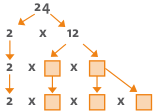
\includegraphics[scale=.75]{Images/diagramadel24.png} 
\end{minipage}\hfill
\begin{minipage}{.5\textwidth}
\begin{align*}
24=&2\times 12\\
24=&2\times \square \times \square = 4 \times \square \\
24=&2\times \square \times \square \times 3=\square \times 3
\end{align*}
\end{minipage}
\end{itemize}
Los números que aparecen en el diagrama son los factores
de 24.

Este diagrama se conoce como diagrama de árbol.

En tu cuaderno, divide a 24 entre cada uno de sus factores.
¿Cómo son las divisiones?

Los números 2 y 12, 4 y 6, 6, 3 y 8 también son divisores de
24. Solo faltan en la lista los número 1 y 24.\\

Responde: ¿Cuándo un número es divisor de otro?
\section*{Ejercito lo aprendido}
Trabaja con dos compañeras o compañeros y respondan las siguientes preguntas o realicen las actividades en el cuaderno.
\begin{enumerate}
\item ¿Es posible saber cuántos elementos tiene el conjunto de múltiplos de un número? Expliquen su respuesta.
\item Completen el diagrama del 2 y el diagrama del 4

\begin{tikzpicture}
[level distance=10mm,
every node/.style={fill=red!60,circle,inner sep=1pt},
level 1/.style={sibling distance=16mm,nodes={fill=red!45}},
level 2/.style={sibling distance=8mm,nodes={fill=red!30}},
level 3/.style={sibling distance=4mm,nodes={fill=red!25}}]
\node {\textbf{2}}
child {node {$\times$}
child {node{0}
child {node{0}}}
child {node{1}
child {node{2}}}
child {node{2}
child {node{4}}}
child {node{3}
child {node{?}}}
child {node{4}
child {node{?}}}
child {node{5}
child {node{?}}}
child {node{6}
child {node{?}}}
child {node{7}
child {node{?}}}
child {node{8}
child {node{?}}}
child {node{9}
child {node{?}}}
child {node{10}
child {node{?}}}
};
\end{tikzpicture}
\end{enumerate}
\end{document}
